\documentclass[twoside]{book}

% Packages required by doxygen
\usepackage{calc}
\usepackage{doxygen}
\usepackage{graphicx}
\usepackage[utf8]{inputenc}
\usepackage{makeidx}
\usepackage{multicol}
\usepackage{multirow}
\usepackage{textcomp}
\usepackage[table]{xcolor}

% Font selection
\usepackage[T1]{fontenc}
\usepackage{mathptmx}
\usepackage[scaled=.90]{helvet}
\usepackage{courier}
\usepackage{amssymb}
\usepackage{sectsty}
\renewcommand{\familydefault}{\sfdefault}
\allsectionsfont{%
  \fontseries{bc}\selectfont%
  \color{darkgray}%
}
\renewcommand{\DoxyLabelFont}{%
  \fontseries{bc}\selectfont%
  \color{darkgray}%
}

% Page & text layout
\usepackage{geometry}
\geometry{%
  a4paper,%
  top=2.5cm,%
  bottom=2.5cm,%
  left=2.5cm,%
  right=2.5cm%
}
\tolerance=750
\hfuzz=15pt
\hbadness=750
\setlength{\emergencystretch}{15pt}
\setlength{\parindent}{0cm}
\setlength{\parskip}{0.2cm}
\makeatletter
\renewcommand{\paragraph}{%
  \@startsection{paragraph}{4}{0ex}{-1.0ex}{1.0ex}{%
    \normalfont\normalsize\bfseries\SS@parafont%
  }%
}
\renewcommand{\subparagraph}{%
  \@startsection{subparagraph}{5}{0ex}{-1.0ex}{1.0ex}{%
    \normalfont\normalsize\bfseries\SS@subparafont%
  }%
}
\makeatother

% Headers & footers
\usepackage{fancyhdr}
\pagestyle{fancyplain}
\fancyhead[LE]{\fancyplain{}{\bfseries\thepage}}
\fancyhead[CE]{\fancyplain{}{}}
\fancyhead[RE]{\fancyplain{}{\bfseries\leftmark}}
\fancyhead[LO]{\fancyplain{}{\bfseries\rightmark}}
\fancyhead[CO]{\fancyplain{}{}}
\fancyhead[RO]{\fancyplain{}{\bfseries\thepage}}
\fancyfoot[LE]{\fancyplain{}{}}
\fancyfoot[CE]{\fancyplain{}{}}
\fancyfoot[RE]{\fancyplain{}{\bfseries\scriptsize Generated on Mon Oct 6 2014 14\-:51\-:04 for Golf Database Server by Doxygen }}
\fancyfoot[LO]{\fancyplain{}{\bfseries\scriptsize Generated on Mon Oct 6 2014 14\-:51\-:04 for Golf Database Server by Doxygen }}
\fancyfoot[CO]{\fancyplain{}{}}
\fancyfoot[RO]{\fancyplain{}{}}
\renewcommand{\footrulewidth}{0.4pt}
\renewcommand{\chaptermark}[1]{%
  \markboth{#1}{}%
}
\renewcommand{\sectionmark}[1]{%
  \markright{\thesection\ #1}%
}

% Indices & bibliography
\usepackage{natbib}
\usepackage[titles]{tocloft}
\setcounter{tocdepth}{3}
\setcounter{secnumdepth}{5}
\makeindex

% Hyperlinks (required, but should be loaded last)
\usepackage{ifpdf}
\ifpdf
  \usepackage[pdftex,pagebackref=true]{hyperref}
\else
  \usepackage[ps2pdf,pagebackref=true]{hyperref}
\fi
\hypersetup{%
  colorlinks=true,%
  linkcolor=blue,%
  citecolor=blue,%
  unicode%
}

% Custom commands
\newcommand{\clearemptydoublepage}{%
  \newpage{\pagestyle{empty}\cleardoublepage}%
}


%===== C O N T E N T S =====

\begin{document}

% Titlepage & ToC
\hypersetup{pageanchor=false}
\pagenumbering{roman}
\begin{titlepage}
\vspace*{7cm}
\begin{center}%
{\Large Golf Database Server \\[1ex]\large 1.\-0 }\\
\vspace*{1cm}
{\large Generated by Doxygen 1.8.6}\\
\vspace*{0.5cm}
{\small Mon Oct 6 2014 14:51:04}\\
\end{center}
\end{titlepage}
\clearemptydoublepage
\tableofcontents
\clearemptydoublepage
\pagenumbering{arabic}
\hypersetup{pageanchor=true}

%--- Begin generated contents ---
\chapter{Hierarchical Index}
\section{Class Hierarchy}
This inheritance list is sorted roughly, but not completely, alphabetically\-:\begin{DoxyCompactList}
\item \contentsline{section}{Db}{\pageref{class_db}}{}
\item \contentsline{section}{Table}{\pageref{class_table}}{}
\begin{DoxyCompactList}
\item \contentsline{section}{City}{\pageref{class_city}}{}
\item \contentsline{section}{Poi}{\pageref{class_poi}}{}
\end{DoxyCompactList}
\end{DoxyCompactList}

\chapter{Data Structure Index}
\section{Data Structures}
Here are the data structures with brief descriptions\-:\begin{DoxyCompactList}
\item\contentsline{section}{\hyperlink{class_city}{City} \\*This class represents the \hyperlink{class_city}{City} table }{\pageref{class_city}}{}
\item\contentsline{section}{\hyperlink{class_db}{Db} \\*This class allows the connection, access and disconnection of database }{\pageref{class_db}}{}
\item\contentsline{section}{\hyperlink{class_poi}{Poi} \\*This class represents the P\-O\-I table }{\pageref{class_poi}}{}
\item\contentsline{section}{\hyperlink{class_table}{Table} \\*This class contains functions to read/write/delete from the database  }{\pageref{class_table}}{}
\end{DoxyCompactList}

\chapter{File Index}
\section{File List}
Here is a list of all files with brief descriptions\-:\begin{DoxyCompactList}
\item\contentsline{section}{lib/\hyperlink{_city_8php}{City.\-php} \\*This class represents the \hyperlink{class_city}{City} table }{\pageref{_city_8php}}{}
\item\contentsline{section}{lib/\hyperlink{_db_8php}{Db.\-php} \\*\hyperlink{class_db}{Db} class. This class allows the connection, access and disconnection of database }{\pageref{_db_8php}}{}
\item\contentsline{section}{lib/\hyperlink{_poi_8php}{Poi.\-php} \\*This class represents the P\-O\-I table }{\pageref{_poi_8php}}{}
\item\contentsline{section}{lib/\hyperlink{_table_8php}{Table.\-php} \\*This class contains functions to read/write/delete from the database }{\pageref{_table_8php}}{}
\item\contentsline{section}{poi/\hyperlink{nearest_8php}{nearest.\-php} \\*Return nearest city and nearest poi of input coordinates }{\pageref{nearest_8php}}{}
\item\contentsline{section}{populatedb/\hyperlink{extract_camping_8php}{extract\-Camping.\-php} \\*Preparation of a text file to insert list of Camping in France in the database }{\pageref{extract_camping_8php}}{}
\item\contentsline{section}{populatedb/\hyperlink{extract_chateau_8php}{extract\-Chateau.\-php} \\*Preparation of a text file to insert list of castles in France in the database }{\pageref{extract_chateau_8php}}{}
\item\contentsline{section}{populatedb/\hyperlink{extract_golf_8php}{extract\-Golf.\-php} \\*Preparation of a text file to insert list of golf in France in the database }{\pageref{extract_golf_8php}}{}
\item\contentsline{section}{populatedb/\hyperlink{extract_mcdo_8php}{extract\-Mcdo.\-php} \\*Preparation of a text file to insert list of Mcdo in France in the database }{\pageref{extract_mcdo_8php}}{}
\end{DoxyCompactList}

\chapter{Data Structure Documentation}
\hypertarget{class_city}{\section{City Class Reference}
\label{class_city}\index{City@{City}}
}


This class represents the \hyperlink{class_city}{City} table.  




Inheritance diagram for City\-:\nopagebreak
\begin{figure}[H]
\begin{center}
\leavevmode
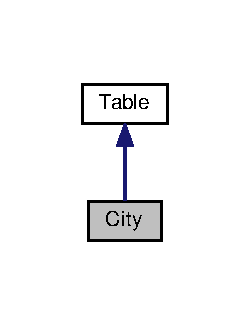
\includegraphics[width=120pt]{class_city__inherit__graph}
\end{center}
\end{figure}


Collaboration diagram for City\-:\nopagebreak
\begin{figure}[H]
\begin{center}
\leavevmode
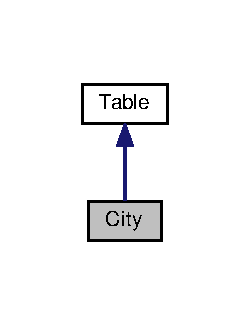
\includegraphics[width=120pt]{class_city__coll__graph}
\end{center}
\end{figure}
\subsection*{Public Member Functions}
\begin{DoxyCompactItemize}
\item 
\hyperlink{class_city_a095c5d389db211932136b53f25f39685}{\-\_\-\-\_\-construct} ()
\item 
\hyperlink{class_city_a4548afef906c15095654cc937f08c49d}{get\-Nearest\-City} (\$longitude, \$latitude, \$population)
\end{DoxyCompactItemize}
\subsection*{Additional Inherited Members}


\subsection{Detailed Description}
This class represents the \hyperlink{class_city}{City} table. 

\subsection{Constructor \& Destructor Documentation}
\hypertarget{class_city_a095c5d389db211932136b53f25f39685}{\index{City@{City}!\-\_\-\-\_\-construct@{\-\_\-\-\_\-construct}}
\index{\-\_\-\-\_\-construct@{\-\_\-\-\_\-construct}!City@{City}}
\subsubsection[{\-\_\-\-\_\-construct}]{\setlength{\rightskip}{0pt plus 5cm}\-\_\-\-\_\-construct (
\begin{DoxyParamCaption}
{}
\end{DoxyParamCaption}
)}}\label{class_city_a095c5d389db211932136b53f25f39685}


\subsection{Member Function Documentation}
\hypertarget{class_city_a4548afef906c15095654cc937f08c49d}{\index{City@{City}!get\-Nearest\-City@{get\-Nearest\-City}}
\index{get\-Nearest\-City@{get\-Nearest\-City}!City@{City}}
\subsubsection[{get\-Nearest\-City}]{\setlength{\rightskip}{0pt plus 5cm}get\-Nearest\-City (
\begin{DoxyParamCaption}
\item[{}]{\$longitude, }
\item[{}]{\$latitude, }
\item[{}]{\$population}
\end{DoxyParamCaption}
)}}\label{class_city_a4548afef906c15095654cc937f08c49d}
This function will search the nearest city coordinates input 
\begin{DoxyParams}{Parameters}
{\em \$longitude} & Longitude of the ball. \\
\hline
{\em \$latitude} & Latitude of the ball. \\
\hline
{\em \$population} & Filter to display small or large cities. \\
\hline
\end{DoxyParams}
\begin{DoxyReturn}{Returns}
\$response Array of nearest city informations 
\end{DoxyReturn}


The documentation for this class was generated from the following file\-:\begin{DoxyCompactItemize}
\item 
lib/\hyperlink{_city_8php}{City.\-php}\end{DoxyCompactItemize}

\hypertarget{class_db}{\section{Db Class Reference}
\label{class_db}\index{Db@{Db}}
}
\subsection*{Public Member Functions}
\begin{DoxyCompactItemize}
\item 
\hyperlink{class_db_a095c5d389db211932136b53f25f39685}{\-\_\-\-\_\-construct} ()
\item 
\hyperlink{class_db_ab550a8a6e40209759ef0459755bb59d9}{get\-Response} (\$query)
\item 
\hyperlink{class_db_a58e50f00fd314af4f7d45fd13015d0b8}{execute\-Query} (\$query)
\item 
\hyperlink{class_db_a8859086080e2f0299818385333705929}{show\-Tables} ()
\item 
\hyperlink{class_db_a8a406dace7e7ab080d58066e627c6465}{deconnect} ()
\end{DoxyCompactItemize}


\subsection{Constructor \& Destructor Documentation}
\hypertarget{class_db_a095c5d389db211932136b53f25f39685}{\index{Db@{Db}!\-\_\-\-\_\-construct@{\-\_\-\-\_\-construct}}
\index{\-\_\-\-\_\-construct@{\-\_\-\-\_\-construct}!Db@{Db}}
\subsubsection[{\-\_\-\-\_\-construct}]{\setlength{\rightskip}{0pt plus 5cm}\-\_\-\-\_\-construct (
\begin{DoxyParamCaption}
{}
\end{DoxyParamCaption}
)}}\label{class_db_a095c5d389db211932136b53f25f39685}


\subsection{Member Function Documentation}
\hypertarget{class_db_a8a406dace7e7ab080d58066e627c6465}{\index{Db@{Db}!deconnect@{deconnect}}
\index{deconnect@{deconnect}!Db@{Db}}
\subsubsection[{deconnect}]{\setlength{\rightskip}{0pt plus 5cm}deconnect (
\begin{DoxyParamCaption}
{}
\end{DoxyParamCaption}
)}}\label{class_db_a8a406dace7e7ab080d58066e627c6465}
Database deconnection \hypertarget{class_db_a58e50f00fd314af4f7d45fd13015d0b8}{\index{Db@{Db}!execute\-Query@{execute\-Query}}
\index{execute\-Query@{execute\-Query}!Db@{Db}}
\subsubsection[{execute\-Query}]{\setlength{\rightskip}{0pt plus 5cm}execute\-Query (
\begin{DoxyParamCaption}
\item[{}]{\$query}
\end{DoxyParamCaption}
)}}\label{class_db_a58e50f00fd314af4f7d45fd13015d0b8}
Returns the result of a sql query 
\begin{DoxyParams}{Parameters}
{\em \$query} & S\-Q\-L request \\
\hline
\end{DoxyParams}
\begin{DoxyReturn}{Returns}
\$response response of query 
\end{DoxyReturn}
\hypertarget{class_db_ab550a8a6e40209759ef0459755bb59d9}{\index{Db@{Db}!get\-Response@{get\-Response}}
\index{get\-Response@{get\-Response}!Db@{Db}}
\subsubsection[{get\-Response}]{\setlength{\rightskip}{0pt plus 5cm}get\-Response (
\begin{DoxyParamCaption}
\item[{}]{\$query}
\end{DoxyParamCaption}
)}}\label{class_db_ab550a8a6e40209759ef0459755bb59d9}
Returns the result of a sql query 
\begin{DoxyParams}{Parameters}
{\em \$query} & S\-Q\-L request \\
\hline
\end{DoxyParams}
\begin{DoxyReturn}{Returns}
\$response response of query 
\end{DoxyReturn}
\hypertarget{class_db_a8859086080e2f0299818385333705929}{\index{Db@{Db}!show\-Tables@{show\-Tables}}
\index{show\-Tables@{show\-Tables}!Db@{Db}}
\subsubsection[{show\-Tables}]{\setlength{\rightskip}{0pt plus 5cm}show\-Tables (
\begin{DoxyParamCaption}
{}
\end{DoxyParamCaption}
)}}\label{class_db_a8859086080e2f0299818385333705929}
Display the list of tables 

The documentation for this class was generated from the following file\-:\begin{DoxyCompactItemize}
\item 
lib/\hyperlink{_db_8php}{Db.\-php}\end{DoxyCompactItemize}

\hypertarget{class_poi}{\section{Poi Class Reference}
\label{class_poi}\index{Poi@{Poi}}
}


Inheritance diagram for Poi\-:\nopagebreak
\begin{figure}[H]
\begin{center}
\leavevmode
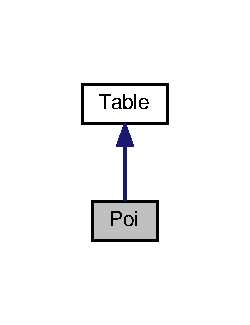
\includegraphics[width=120pt]{class_poi__inherit__graph}
\end{center}
\end{figure}


Collaboration diagram for Poi\-:\nopagebreak
\begin{figure}[H]
\begin{center}
\leavevmode
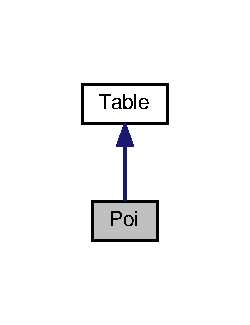
\includegraphics[width=120pt]{class_poi__coll__graph}
\end{center}
\end{figure}
\subsection*{Public Member Functions}
\begin{DoxyCompactItemize}
\item 
\hyperlink{class_poi_a095c5d389db211932136b53f25f39685}{\-\_\-\-\_\-construct} ()
\item 
\hyperlink{class_poi_a4b46f688fae9d9a5cad7cabb2d579794}{get\-Nearest\-Poi} (\$longitude, \$latitude, \$limit\-\_\-km)
\end{DoxyCompactItemize}
\subsection*{Additional Inherited Members}


\subsection{Constructor \& Destructor Documentation}
\hypertarget{class_poi_a095c5d389db211932136b53f25f39685}{\index{Poi@{Poi}!\-\_\-\-\_\-construct@{\-\_\-\-\_\-construct}}
\index{\-\_\-\-\_\-construct@{\-\_\-\-\_\-construct}!Poi@{Poi}}
\subsubsection[{\-\_\-\-\_\-construct}]{\setlength{\rightskip}{0pt plus 5cm}\-\_\-\-\_\-construct (
\begin{DoxyParamCaption}
{}
\end{DoxyParamCaption}
)}}\label{class_poi_a095c5d389db211932136b53f25f39685}


\subsection{Member Function Documentation}
\hypertarget{class_poi_a4b46f688fae9d9a5cad7cabb2d579794}{\index{Poi@{Poi}!get\-Nearest\-Poi@{get\-Nearest\-Poi}}
\index{get\-Nearest\-Poi@{get\-Nearest\-Poi}!Poi@{Poi}}
\subsubsection[{get\-Nearest\-Poi}]{\setlength{\rightskip}{0pt plus 5cm}get\-Nearest\-Poi (
\begin{DoxyParamCaption}
\item[{}]{\$longitude, }
\item[{}]{\$latitude, }
\item[{}]{\$limit\-\_\-km}
\end{DoxyParamCaption}
)}}\label{class_poi_a4b46f688fae9d9a5cad7cabb2d579794}
This function will search the nearest poi of input coordinates. 
\begin{DoxyParams}{Parameters}
{\em \$longitude} & Longitude of the ball. \\
\hline
{\em \$latitude} & Latitude of the ball. \\
\hline
{\em \$limit\-\_\-km} & Defines the scope of \hyperlink{class_poi}{Poi} display. \\
\hline
\end{DoxyParams}
\begin{DoxyReturn}{Returns}
\$response Array of nearest poi informations 
\end{DoxyReturn}


The documentation for this class was generated from the following file\-:\begin{DoxyCompactItemize}
\item 
lib/\hyperlink{_poi_8php}{Poi.\-php}\end{DoxyCompactItemize}

\hypertarget{class_table}{\section{Table Class Reference}
\label{class_table}\index{Table@{Table}}
}


This class contains functions to read/write/delete from the database.  




Inheritance diagram for Table\-:\nopagebreak
\begin{figure}[H]
\begin{center}
\leavevmode
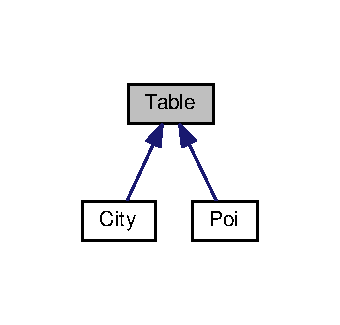
\includegraphics[width=163pt]{class_table__inherit__graph}
\end{center}
\end{figure}
\subsection*{Public Member Functions}
\begin{DoxyCompactItemize}
\item 
\hyperlink{class_table_aba0d5b303383fb5b1fabb5fd01cd3800}{get\-All} ()
\begin{DoxyCompactList}\small\item\em This function returns the entire table. \end{DoxyCompactList}\item 
\hyperlink{class_table_a2f4379fc75908df9538e80a8a7f1043a}{get\-Rows} (\$cond)
\begin{DoxyCompactList}\small\item\em Collect some tuples of a table after some content provided \$cond table. \end{DoxyCompactList}\item 
\hyperlink{class_table_a60590b38a52542f17a63f5211ba3a111}{insert\-Row} (\$valeurs)
\item 
\hyperlink{class_table_a9d23647d9285ae7c3066280c9ad2bf9f}{delete\-Row} (\$cond)
\item 
\hyperlink{class_table_a3ee38d1ab83f5834b5ffeae8daad85f8}{update\-Row} (\$new\-Value, \$cond)
\item 
\hyperlink{class_table_a8a406dace7e7ab080d58066e627c6465}{deconnect} ()
\end{DoxyCompactItemize}
\subsection*{Protected Attributes}
\begin{DoxyCompactItemize}
\item 
\hyperlink{class_table_a1fa3127fc82f96b1436d871ef02be319}{\$db}
\begin{DoxyCompactList}\small\item\em Database. \end{DoxyCompactList}\item 
\hyperlink{class_table_ab2fc40d43824ea3e1ce5d86dee0d763b}{\$name}
\begin{DoxyCompactList}\small\item\em table name \end{DoxyCompactList}\item 
\hyperlink{class_table_ab2303c817e3b402b77b7f99627b9c319}{\$fields}
\end{DoxyCompactItemize}


\subsection{Detailed Description}
This class contains functions to read/write/delete from the database. 

\subsection{Member Function Documentation}
\hypertarget{class_table_a8a406dace7e7ab080d58066e627c6465}{\index{Table@{Table}!deconnect@{deconnect}}
\index{deconnect@{deconnect}!Table@{Table}}
\subsubsection[{deconnect}]{\setlength{\rightskip}{0pt plus 5cm}deconnect (
\begin{DoxyParamCaption}
{}
\end{DoxyParamCaption}
)}}\label{class_table_a8a406dace7e7ab080d58066e627c6465}
Database deconnect \hypertarget{class_table_a9d23647d9285ae7c3066280c9ad2bf9f}{\index{Table@{Table}!delete\-Row@{delete\-Row}}
\index{delete\-Row@{delete\-Row}!Table@{Table}}
\subsubsection[{delete\-Row}]{\setlength{\rightskip}{0pt plus 5cm}delete\-Row (
\begin{DoxyParamCaption}
\item[{}]{\$cond}
\end{DoxyParamCaption}
)}}\label{class_table_a9d23647d9285ae7c3066280c9ad2bf9f}
Delete rows into a table according to conditions 
\begin{DoxyParams}{Parameters}
{\em \$cond} & delete condition \\
\hline
\end{DoxyParams}
\begin{DoxyReturn}{Returns}
0 
\end{DoxyReturn}
\hypertarget{class_table_aba0d5b303383fb5b1fabb5fd01cd3800}{\index{Table@{Table}!get\-All@{get\-All}}
\index{get\-All@{get\-All}!Table@{Table}}
\subsubsection[{get\-All}]{\setlength{\rightskip}{0pt plus 5cm}get\-All (
\begin{DoxyParamCaption}
{}
\end{DoxyParamCaption}
)}}\label{class_table_aba0d5b303383fb5b1fabb5fd01cd3800}


This function returns the entire table. 

\begin{DoxyReturn}{Returns}
\$all\-Rows Data list 
\end{DoxyReturn}
\hypertarget{class_table_a2f4379fc75908df9538e80a8a7f1043a}{\index{Table@{Table}!get\-Rows@{get\-Rows}}
\index{get\-Rows@{get\-Rows}!Table@{Table}}
\subsubsection[{get\-Rows}]{\setlength{\rightskip}{0pt plus 5cm}get\-Rows (
\begin{DoxyParamCaption}
\item[{}]{\$cond}
\end{DoxyParamCaption}
)}}\label{class_table_a2f4379fc75908df9538e80a8a7f1043a}


Collect some tuples of a table after some content provided \$cond table. 


\begin{DoxyParams}{Parameters}
{\em \$cond} & select conditions \\
\hline
\end{DoxyParams}
\begin{DoxyReturn}{Returns}
\$rows Data list 
\end{DoxyReturn}
\hypertarget{class_table_a60590b38a52542f17a63f5211ba3a111}{\index{Table@{Table}!insert\-Row@{insert\-Row}}
\index{insert\-Row@{insert\-Row}!Table@{Table}}
\subsubsection[{insert\-Row}]{\setlength{\rightskip}{0pt plus 5cm}insert\-Row (
\begin{DoxyParamCaption}
\item[{}]{\$valeurs}
\end{DoxyParamCaption}
)}}\label{class_table_a60590b38a52542f17a63f5211ba3a111}
Inserting rows into a table 
\begin{DoxyParams}{Parameters}
{\em \$valeurs} & value list to insert \\
\hline
\end{DoxyParams}
\begin{DoxyReturn}{Returns}
\$id\-Insere id of the inserted row 
\end{DoxyReturn}
\hypertarget{class_table_a3ee38d1ab83f5834b5ffeae8daad85f8}{\index{Table@{Table}!update\-Row@{update\-Row}}
\index{update\-Row@{update\-Row}!Table@{Table}}
\subsubsection[{update\-Row}]{\setlength{\rightskip}{0pt plus 5cm}update\-Row (
\begin{DoxyParamCaption}
\item[{}]{\$new\-Value, }
\item[{}]{\$cond}
\end{DoxyParamCaption}
)}}\label{class_table_a3ee38d1ab83f5834b5ffeae8daad85f8}
Update rows into a table according to conditions 
\begin{DoxyParams}{Parameters}
{\em \$new\-Value} & update value \\
\hline
{\em \$cond} & update condition \\
\hline
\end{DoxyParams}
\begin{DoxyReturn}{Returns}
-\/1 if problem 
\end{DoxyReturn}


\subsection{Field Documentation}
\hypertarget{class_table_a1fa3127fc82f96b1436d871ef02be319}{\index{Table@{Table}!\$db@{\$db}}
\index{\$db@{\$db}!Table@{Table}}
\subsubsection[{\$db}]{\setlength{\rightskip}{0pt plus 5cm}\$db\hspace{0.3cm}{\ttfamily [protected]}}}\label{class_table_a1fa3127fc82f96b1436d871ef02be319}


Database. 

\hypertarget{class_table_ab2303c817e3b402b77b7f99627b9c319}{\index{Table@{Table}!\$fields@{\$fields}}
\index{\$fields@{\$fields}!Table@{Table}}
\subsubsection[{\$fields}]{\setlength{\rightskip}{0pt plus 5cm}\$fields\hspace{0.3cm}{\ttfamily [protected]}}}\label{class_table_ab2303c817e3b402b77b7f99627b9c319}
\hypertarget{class_table_ab2fc40d43824ea3e1ce5d86dee0d763b}{\index{Table@{Table}!\$name@{\$name}}
\index{\$name@{\$name}!Table@{Table}}
\subsubsection[{\$name}]{\setlength{\rightskip}{0pt plus 5cm}\$name\hspace{0.3cm}{\ttfamily [protected]}}}\label{class_table_ab2fc40d43824ea3e1ce5d86dee0d763b}


table name 



The documentation for this class was generated from the following file\-:\begin{DoxyCompactItemize}
\item 
lib/\hyperlink{_table_8php}{Table.\-php}\end{DoxyCompactItemize}

\chapter{File Documentation}
\hypertarget{_city_8php}{\section{lib/\-City.php File Reference}
\label{_city_8php}\index{lib/\-City.\-php@{lib/\-City.\-php}}
}


\hyperlink{class_city}{City} class.  


\subsection*{Data Structures}
\begin{DoxyCompactItemize}
\item 
class \hyperlink{class_city}{City}
\end{DoxyCompactItemize}


\subsection{Detailed Description}
\hyperlink{class_city}{City} class. \begin{DoxyAuthor}{Author}
Loïc T\-R\-I\-C\-J\-A\-U\-D 
\end{DoxyAuthor}
\begin{DoxyVersion}{Version}
1.\-0 
\end{DoxyVersion}
\begin{DoxyDate}{Date}
01/10/2014 
\end{DoxyDate}

\hypertarget{_db_8php}{\section{lib/\-Db.php File Reference}
\label{_db_8php}\index{lib/\-Db.\-php@{lib/\-Db.\-php}}
}


\hyperlink{class_db}{Db} class. This class allows the connection, access and disconnection of database.  


\subsection*{Data Structures}
\begin{DoxyCompactItemize}
\item 
class \hyperlink{class_db}{Db}
\end{DoxyCompactItemize}


\subsection{Detailed Description}
\hyperlink{class_db}{Db} class. This class allows the connection, access and disconnection of database. \begin{DoxyAuthor}{Author}
Loïc T\-R\-I\-C\-J\-A\-U\-D 
\end{DoxyAuthor}
\begin{DoxyVersion}{Version}
1.\-0 
\end{DoxyVersion}
\begin{DoxyDate}{Date}
01/10/2014 
\end{DoxyDate}

\hypertarget{_poi_8php}{\section{lib/\-Poi.php File Reference}
\label{_poi_8php}\index{lib/\-Poi.\-php@{lib/\-Poi.\-php}}
}


This class represents the P\-O\-I table.  


\subsection*{Data Structures}
\begin{DoxyCompactItemize}
\item 
class \hyperlink{class_poi}{Poi}
\begin{DoxyCompactList}\small\item\em This class represents the P\-O\-I table. \end{DoxyCompactList}\end{DoxyCompactItemize}


\subsection{Detailed Description}
This class represents the P\-O\-I table. \begin{DoxyAuthor}{Author}
Loïc T\-R\-I\-C\-J\-A\-U\-D 
\end{DoxyAuthor}
\begin{DoxyVersion}{Version}
1.\-0 
\end{DoxyVersion}
\begin{DoxyDate}{Date}
01/10/2014 
\end{DoxyDate}

\hypertarget{_table_8php}{\section{lib/\-Table.php File Reference}
\label{_table_8php}\index{lib/\-Table.\-php@{lib/\-Table.\-php}}
}
\subsection*{Data Structures}
\begin{DoxyCompactItemize}
\item 
class \hyperlink{class_table}{Table}
\begin{DoxyCompactList}\small\item\em This class contains functions to read/write/delete from the database. \end{DoxyCompactList}\end{DoxyCompactItemize}


\subsection{Detailed Description}
\begin{DoxyAuthor}{Author}
Loïc T\-R\-I\-C\-J\-A\-U\-D 
\end{DoxyAuthor}
\begin{DoxyVersion}{Version}
1.\-0 
\end{DoxyVersion}
\begin{DoxyDate}{Date}
01/10/2014 
\end{DoxyDate}

\hypertarget{nearest_8php}{\section{poi/nearest.php File Reference}
\label{nearest_8php}\index{poi/nearest.\-php@{poi/nearest.\-php}}
}


Return nearest city and nearest poi of input coordinates.  


\subsection*{Variables}
\begin{DoxyCompactItemize}
\item 
\hyperlink{nearest_8php_aabb5b5c018fed3789fce382e336cfa47}{\$longitude} = \$\-\_\-\-G\-E\-T\mbox{[}'lg'\mbox{]}
\begin{DoxyCompactList}\small\item\em Longitude retrieving in the url. \end{DoxyCompactList}\item 
\hyperlink{nearest_8php_a5635a7326fb0b96e184ca6f5baa13e94}{\$latitude} = \$\-\_\-\-G\-E\-T\mbox{[}'lt'\mbox{]}
\begin{DoxyCompactList}\small\item\em Latitude retrieving in the url. \end{DoxyCompactList}\item 
\hyperlink{nearest_8php_afc1939ed7d0e8629546e2bc27b02dbc1}{\$population} = 3000
\begin{DoxyCompactList}\small\item\em Filter population to display small or large cities. \end{DoxyCompactList}\item 
\hyperlink{nearest_8php_a00de150c5780d1d74512d2f6c6477d22}{\$limit\-\_\-km} = 30
\begin{DoxyCompactList}\small\item\em Limit of kilometers of P\-O\-I. \end{DoxyCompactList}\item 
\hyperlink{nearest_8php_a5b9ddd3e3a69d8901270064346bdef49}{\$city} = new \hyperlink{class_city}{City}()
\item 
\hyperlink{nearest_8php_ad20bfb1568497d36431fbd90847417cc}{\$array\-\_\-nearest\-\_\-city} = \$city-\/$>$get\-Nearest\-City(\$longitude,\$latitude,\$population)
\item 
\hyperlink{nearest_8php_a15278c25ad2a899afd235d0093857e4c}{\$poi} = new \hyperlink{class_poi}{Poi}()
\item 
\hyperlink{nearest_8php_a0919b64d32b8806e2d59272d197f32e7}{\$array\-\_\-nearest\-\_\-poi} = \$poi-\/$>$get\-Nearest\-Poi(\$longitude,\$latitude,\$limit\-\_\-km)
\item 
\hyperlink{nearest_8php_abf6b27fab4f9b20ea05f510f3b597d52}{\$nearest\-\_\-city}
\item 
\hyperlink{nearest_8php_a0b142ae8ff992c1fff670c905b46e066}{\$nearest\-\_\-city\-\_\-json} = json\-\_\-encode(\$nearest\-\_\-city, J\-S\-O\-N\-\_\-\-U\-N\-E\-S\-C\-A\-P\-E\-D\-\_\-\-U\-N\-I\-C\-O\-D\-E $\vert$ J\-S\-O\-N\-\_\-\-U\-N\-E\-S\-C\-A\-P\-E\-D\-\_\-\-S\-L\-A\-S\-H\-E\-S)
\end{DoxyCompactItemize}


\subsection{Detailed Description}
Return nearest city and nearest poi of input coordinates. \begin{DoxyAuthor}{Author}
Loïc T\-R\-I\-C\-J\-A\-U\-D 
\end{DoxyAuthor}
\begin{DoxyVersion}{Version}
1.\-0 
\end{DoxyVersion}
\begin{DoxyDate}{Date}
01/10/2014 
\end{DoxyDate}


\subsection{Variable Documentation}
\hypertarget{nearest_8php_ad20bfb1568497d36431fbd90847417cc}{\index{nearest.\-php@{nearest.\-php}!\$array\-\_\-nearest\-\_\-city@{\$array\-\_\-nearest\-\_\-city}}
\index{\$array\-\_\-nearest\-\_\-city@{\$array\-\_\-nearest\-\_\-city}!nearest.php@{nearest.\-php}}
\subsubsection[{\$array\-\_\-nearest\-\_\-city}]{\setlength{\rightskip}{0pt plus 5cm}\$array\-\_\-nearest\-\_\-city = \$city-\/$>$get\-Nearest\-City(\$longitude,\$latitude,\$population)}}\label{nearest_8php_ad20bfb1568497d36431fbd90847417cc}
\hypertarget{nearest_8php_a0919b64d32b8806e2d59272d197f32e7}{\index{nearest.\-php@{nearest.\-php}!\$array\-\_\-nearest\-\_\-poi@{\$array\-\_\-nearest\-\_\-poi}}
\index{\$array\-\_\-nearest\-\_\-poi@{\$array\-\_\-nearest\-\_\-poi}!nearest.php@{nearest.\-php}}
\subsubsection[{\$array\-\_\-nearest\-\_\-poi}]{\setlength{\rightskip}{0pt plus 5cm}\$array\-\_\-nearest\-\_\-poi = \$poi-\/$>$get\-Nearest\-Poi(\$longitude,\$latitude,\$limit\-\_\-km)}}\label{nearest_8php_a0919b64d32b8806e2d59272d197f32e7}
\hypertarget{nearest_8php_a5b9ddd3e3a69d8901270064346bdef49}{\index{nearest.\-php@{nearest.\-php}!\$city@{\$city}}
\index{\$city@{\$city}!nearest.php@{nearest.\-php}}
\subsubsection[{\$city}]{\setlength{\rightskip}{0pt plus 5cm}\$city = new {\bf City}()}}\label{nearest_8php_a5b9ddd3e3a69d8901270064346bdef49}
\hypertarget{nearest_8php_a5635a7326fb0b96e184ca6f5baa13e94}{\index{nearest.\-php@{nearest.\-php}!\$latitude@{\$latitude}}
\index{\$latitude@{\$latitude}!nearest.php@{nearest.\-php}}
\subsubsection[{\$latitude}]{\setlength{\rightskip}{0pt plus 5cm}\$latitude = \$\-\_\-\-G\-E\-T\mbox{[}'lt'\mbox{]}}}\label{nearest_8php_a5635a7326fb0b96e184ca6f5baa13e94}


Latitude retrieving in the url. 

\hypertarget{nearest_8php_a00de150c5780d1d74512d2f6c6477d22}{\index{nearest.\-php@{nearest.\-php}!\$limit\-\_\-km@{\$limit\-\_\-km}}
\index{\$limit\-\_\-km@{\$limit\-\_\-km}!nearest.php@{nearest.\-php}}
\subsubsection[{\$limit\-\_\-km}]{\setlength{\rightskip}{0pt plus 5cm}\$limit\-\_\-km = 30}}\label{nearest_8php_a00de150c5780d1d74512d2f6c6477d22}


Limit of kilometers of P\-O\-I. 

\hypertarget{nearest_8php_aabb5b5c018fed3789fce382e336cfa47}{\index{nearest.\-php@{nearest.\-php}!\$longitude@{\$longitude}}
\index{\$longitude@{\$longitude}!nearest.php@{nearest.\-php}}
\subsubsection[{\$longitude}]{\setlength{\rightskip}{0pt plus 5cm}\$longitude = \$\-\_\-\-G\-E\-T\mbox{[}'lg'\mbox{]}}}\label{nearest_8php_aabb5b5c018fed3789fce382e336cfa47}


Longitude retrieving in the url. 

\hypertarget{nearest_8php_abf6b27fab4f9b20ea05f510f3b597d52}{\index{nearest.\-php@{nearest.\-php}!\$nearest\-\_\-city@{\$nearest\-\_\-city}}
\index{\$nearest\-\_\-city@{\$nearest\-\_\-city}!nearest.php@{nearest.\-php}}
\subsubsection[{\$nearest\-\_\-city}]{\setlength{\rightskip}{0pt plus 5cm}\$nearest\-\_\-city}}\label{nearest_8php_abf6b27fab4f9b20ea05f510f3b597d52}
{\bfseries Initial value\-:}
\begin{DoxyCode}
= array(
    \textcolor{stringliteral}{"name"} => \hyperlink{nearest_8php_ad20bfb1568497d36431fbd90847417cc}{$array\_nearest\_city}[0][\textcolor{stringliteral}{"ville\_nom\_reel"}],
    \textcolor{stringliteral}{"lg"}   => \hyperlink{nearest_8php_ad20bfb1568497d36431fbd90847417cc}{$array\_nearest\_city}[0][\textcolor{stringliteral}{"ville\_longitude\_deg"}],
    \textcolor{stringliteral}{"lt"}   => \hyperlink{nearest_8php_ad20bfb1568497d36431fbd90847417cc}{$array\_nearest\_city}[0][\textcolor{stringliteral}{"ville\_latitude\_deg"}],
    \textcolor{stringliteral}{"url"}  => \hyperlink{nearest_8php_ad20bfb1568497d36431fbd90847417cc}{$array\_nearest\_city}[0][\textcolor{stringliteral}{"ville\_url\_wiki"}],
    \textcolor{stringliteral}{"listOfPoi"} => \hyperlink{nearest_8php_a0919b64d32b8806e2d59272d197f32e7}{$array\_nearest\_poi}
)
\end{DoxyCode}
\hypertarget{nearest_8php_a0b142ae8ff992c1fff670c905b46e066}{\index{nearest.\-php@{nearest.\-php}!\$nearest\-\_\-city\-\_\-json@{\$nearest\-\_\-city\-\_\-json}}
\index{\$nearest\-\_\-city\-\_\-json@{\$nearest\-\_\-city\-\_\-json}!nearest.php@{nearest.\-php}}
\subsubsection[{\$nearest\-\_\-city\-\_\-json}]{\setlength{\rightskip}{0pt plus 5cm}\$nearest\-\_\-city\-\_\-json = json\-\_\-encode(\$nearest\-\_\-city, J\-S\-O\-N\-\_\-\-U\-N\-E\-S\-C\-A\-P\-E\-D\-\_\-\-U\-N\-I\-C\-O\-D\-E $\vert$ J\-S\-O\-N\-\_\-\-U\-N\-E\-S\-C\-A\-P\-E\-D\-\_\-\-S\-L\-A\-S\-H\-E\-S)}}\label{nearest_8php_a0b142ae8ff992c1fff670c905b46e066}
\hypertarget{nearest_8php_a15278c25ad2a899afd235d0093857e4c}{\index{nearest.\-php@{nearest.\-php}!\$poi@{\$poi}}
\index{\$poi@{\$poi}!nearest.php@{nearest.\-php}}
\subsubsection[{\$poi}]{\setlength{\rightskip}{0pt plus 5cm}\$poi = new {\bf Poi}()}}\label{nearest_8php_a15278c25ad2a899afd235d0093857e4c}
\hypertarget{nearest_8php_afc1939ed7d0e8629546e2bc27b02dbc1}{\index{nearest.\-php@{nearest.\-php}!\$population@{\$population}}
\index{\$population@{\$population}!nearest.php@{nearest.\-php}}
\subsubsection[{\$population}]{\setlength{\rightskip}{0pt plus 5cm}\$population = 3000}}\label{nearest_8php_afc1939ed7d0e8629546e2bc27b02dbc1}


Filter population to display small or large cities. 


\hypertarget{extract_camping_8php}{\section{populatedb/extract\-Camping.php File Reference}
\label{extract_camping_8php}\index{populatedb/extract\-Camping.\-php@{populatedb/extract\-Camping.\-php}}
}


Preparation of a text file to insert list of Camping in France in the database.  


\subsection*{Variables}
\begin{DoxyCompactItemize}
\item 
\hyperlink{extract_camping_8php_aa1bfbd27060176201b271918dff57e8f}{\$file} = fopen(\char`\"{}camping.\-asc\char`\"{}, \char`\"{}r\char`\"{})
\item 
\hyperlink{extract_camping_8php_a711797613cb863ca0756df789c396bf2}{\$host} = \char`\"{}localhost\char`\"{}
\item 
\hyperlink{extract_camping_8php_a598ca4e71b15a1313ec95f0df1027ca5}{\$user} = \char`\"{}root\char`\"{}
\item 
\hyperlink{extract_camping_8php_a94f91e878bce0991e2cd595c5dd79b3f}{\$bdd} = \char`\"{}D\-B\-\_\-\-G\-L\-F\char`\"{}
\item 
\hyperlink{extract_camping_8php_a12e4252e778952d356721bc655cff8c8}{\$pwd} = \char`\"{}\char`\"{}
\item 
\hyperlink{extract_camping_8php_a83018d9153d17d91fbcf3bc10158d34f}{\$i} =0
\item 
\hyperlink{extract_camping_8php_a4eebe21070c3a655a77e55ea3fe137f5}{while} (!feof(\$file))
\end{DoxyCompactItemize}


\subsection{Detailed Description}
Preparation of a text file to insert list of Camping in France in the database. \begin{DoxyAuthor}{Author}
Loïc T\-R\-I\-C\-J\-A\-U\-D 
\end{DoxyAuthor}
\begin{DoxyVersion}{Version}
1.\-0 
\end{DoxyVersion}
\begin{DoxyDate}{Date}
03/10/2014 
\end{DoxyDate}


\subsection{Variable Documentation}
\hypertarget{extract_camping_8php_a94f91e878bce0991e2cd595c5dd79b3f}{\index{extract\-Camping.\-php@{extract\-Camping.\-php}!\$bdd@{\$bdd}}
\index{\$bdd@{\$bdd}!extractCamping.php@{extract\-Camping.\-php}}
\subsubsection[{\$bdd}]{\setlength{\rightskip}{0pt plus 5cm}\$bdd = \char`\"{}D\-B\-\_\-\-G\-L\-F\char`\"{}}}\label{extract_camping_8php_a94f91e878bce0991e2cd595c5dd79b3f}
\hypertarget{extract_camping_8php_aa1bfbd27060176201b271918dff57e8f}{\index{extract\-Camping.\-php@{extract\-Camping.\-php}!\$file@{\$file}}
\index{\$file@{\$file}!extractCamping.php@{extract\-Camping.\-php}}
\subsubsection[{\$file}]{\setlength{\rightskip}{0pt plus 5cm}\$file = fopen(\char`\"{}camping.\-asc\char`\"{}, \char`\"{}r\char`\"{})}}\label{extract_camping_8php_aa1bfbd27060176201b271918dff57e8f}
\hypertarget{extract_camping_8php_a711797613cb863ca0756df789c396bf2}{\index{extract\-Camping.\-php@{extract\-Camping.\-php}!\$host@{\$host}}
\index{\$host@{\$host}!extractCamping.php@{extract\-Camping.\-php}}
\subsubsection[{\$host}]{\setlength{\rightskip}{0pt plus 5cm}\$host = \char`\"{}localhost\char`\"{}}}\label{extract_camping_8php_a711797613cb863ca0756df789c396bf2}
\hypertarget{extract_camping_8php_a83018d9153d17d91fbcf3bc10158d34f}{\index{extract\-Camping.\-php@{extract\-Camping.\-php}!\$i@{\$i}}
\index{\$i@{\$i}!extractCamping.php@{extract\-Camping.\-php}}
\subsubsection[{\$i}]{\setlength{\rightskip}{0pt plus 5cm}\$i =0}}\label{extract_camping_8php_a83018d9153d17d91fbcf3bc10158d34f}
\hypertarget{extract_camping_8php_a12e4252e778952d356721bc655cff8c8}{\index{extract\-Camping.\-php@{extract\-Camping.\-php}!\$pwd@{\$pwd}}
\index{\$pwd@{\$pwd}!extractCamping.php@{extract\-Camping.\-php}}
\subsubsection[{\$pwd}]{\setlength{\rightskip}{0pt plus 5cm}\$pwd = \char`\"{}\char`\"{}}}\label{extract_camping_8php_a12e4252e778952d356721bc655cff8c8}
\hypertarget{extract_camping_8php_a598ca4e71b15a1313ec95f0df1027ca5}{\index{extract\-Camping.\-php@{extract\-Camping.\-php}!\$user@{\$user}}
\index{\$user@{\$user}!extractCamping.php@{extract\-Camping.\-php}}
\subsubsection[{\$user}]{\setlength{\rightskip}{0pt plus 5cm}\$user = \char`\"{}root\char`\"{}}}\label{extract_camping_8php_a598ca4e71b15a1313ec95f0df1027ca5}
\hypertarget{extract_camping_8php_a4eebe21070c3a655a77e55ea3fe137f5}{\index{extract\-Camping.\-php@{extract\-Camping.\-php}!while@{while}}
\index{while@{while}!extractCamping.php@{extract\-Camping.\-php}}
\subsubsection[{while}]{\setlength{\rightskip}{0pt plus 5cm}while(!feof(\$file))}}\label{extract_camping_8php_a4eebe21070c3a655a77e55ea3fe137f5}

\hypertarget{extract_chateau_8php}{\section{populatedb/extract\-Chateau.php File Reference}
\label{extract_chateau_8php}\index{populatedb/extract\-Chateau.\-php@{populatedb/extract\-Chateau.\-php}}
}


Preparation of a text file to insert list of castles in France in the database.  


\subsection*{Variables}
\begin{DoxyCompactItemize}
\item 
\hyperlink{extract_chateau_8php_aa1bfbd27060176201b271918dff57e8f}{\$file} = fopen(\char`\"{}chateaux.\-asc\char`\"{}, \char`\"{}r\char`\"{})
\item 
\hyperlink{extract_chateau_8php_a711797613cb863ca0756df789c396bf2}{\$host} = \char`\"{}localhost\char`\"{}
\item 
\hyperlink{extract_chateau_8php_a598ca4e71b15a1313ec95f0df1027ca5}{\$user} = \char`\"{}root\char`\"{}
\item 
\hyperlink{extract_chateau_8php_a94f91e878bce0991e2cd595c5dd79b3f}{\$bdd} = \char`\"{}D\-B\-\_\-\-G\-L\-F\char`\"{}
\item 
\hyperlink{extract_chateau_8php_a12e4252e778952d356721bc655cff8c8}{\$pwd} = \char`\"{}\char`\"{}
\item 
\hyperlink{extract_chateau_8php_a83018d9153d17d91fbcf3bc10158d34f}{\$i} =0
\item 
\hyperlink{extract_chateau_8php_a4eebe21070c3a655a77e55ea3fe137f5}{while} (!feof(\$file))
\end{DoxyCompactItemize}


\subsection{Detailed Description}
Preparation of a text file to insert list of castles in France in the database. \begin{DoxyAuthor}{Author}
Loïc T\-R\-I\-C\-J\-A\-U\-D 
\end{DoxyAuthor}
\begin{DoxyVersion}{Version}
1.\-0 
\end{DoxyVersion}
\begin{DoxyDate}{Date}
05/10/2014 
\end{DoxyDate}


\subsection{Variable Documentation}
\hypertarget{extract_chateau_8php_a94f91e878bce0991e2cd595c5dd79b3f}{\index{extract\-Chateau.\-php@{extract\-Chateau.\-php}!\$bdd@{\$bdd}}
\index{\$bdd@{\$bdd}!extractChateau.php@{extract\-Chateau.\-php}}
\subsubsection[{\$bdd}]{\setlength{\rightskip}{0pt plus 5cm}\$bdd = \char`\"{}D\-B\-\_\-\-G\-L\-F\char`\"{}}}\label{extract_chateau_8php_a94f91e878bce0991e2cd595c5dd79b3f}
\hypertarget{extract_chateau_8php_aa1bfbd27060176201b271918dff57e8f}{\index{extract\-Chateau.\-php@{extract\-Chateau.\-php}!\$file@{\$file}}
\index{\$file@{\$file}!extractChateau.php@{extract\-Chateau.\-php}}
\subsubsection[{\$file}]{\setlength{\rightskip}{0pt plus 5cm}\$file = fopen(\char`\"{}chateaux.\-asc\char`\"{}, \char`\"{}r\char`\"{})}}\label{extract_chateau_8php_aa1bfbd27060176201b271918dff57e8f}
\hypertarget{extract_chateau_8php_a711797613cb863ca0756df789c396bf2}{\index{extract\-Chateau.\-php@{extract\-Chateau.\-php}!\$host@{\$host}}
\index{\$host@{\$host}!extractChateau.php@{extract\-Chateau.\-php}}
\subsubsection[{\$host}]{\setlength{\rightskip}{0pt plus 5cm}\$host = \char`\"{}localhost\char`\"{}}}\label{extract_chateau_8php_a711797613cb863ca0756df789c396bf2}
\hypertarget{extract_chateau_8php_a83018d9153d17d91fbcf3bc10158d34f}{\index{extract\-Chateau.\-php@{extract\-Chateau.\-php}!\$i@{\$i}}
\index{\$i@{\$i}!extractChateau.php@{extract\-Chateau.\-php}}
\subsubsection[{\$i}]{\setlength{\rightskip}{0pt plus 5cm}\$i =0}}\label{extract_chateau_8php_a83018d9153d17d91fbcf3bc10158d34f}
\hypertarget{extract_chateau_8php_a12e4252e778952d356721bc655cff8c8}{\index{extract\-Chateau.\-php@{extract\-Chateau.\-php}!\$pwd@{\$pwd}}
\index{\$pwd@{\$pwd}!extractChateau.php@{extract\-Chateau.\-php}}
\subsubsection[{\$pwd}]{\setlength{\rightskip}{0pt plus 5cm}\$pwd = \char`\"{}\char`\"{}}}\label{extract_chateau_8php_a12e4252e778952d356721bc655cff8c8}
\hypertarget{extract_chateau_8php_a598ca4e71b15a1313ec95f0df1027ca5}{\index{extract\-Chateau.\-php@{extract\-Chateau.\-php}!\$user@{\$user}}
\index{\$user@{\$user}!extractChateau.php@{extract\-Chateau.\-php}}
\subsubsection[{\$user}]{\setlength{\rightskip}{0pt plus 5cm}\$user = \char`\"{}root\char`\"{}}}\label{extract_chateau_8php_a598ca4e71b15a1313ec95f0df1027ca5}
\hypertarget{extract_chateau_8php_a4eebe21070c3a655a77e55ea3fe137f5}{\index{extract\-Chateau.\-php@{extract\-Chateau.\-php}!while@{while}}
\index{while@{while}!extractChateau.php@{extract\-Chateau.\-php}}
\subsubsection[{while}]{\setlength{\rightskip}{0pt plus 5cm}while(!feof(\$file))}}\label{extract_chateau_8php_a4eebe21070c3a655a77e55ea3fe137f5}

\hypertarget{extract_golf_8php}{\section{populatedb/extract\-Golf.php File Reference}
\label{extract_golf_8php}\index{populatedb/extract\-Golf.\-php@{populatedb/extract\-Golf.\-php}}
}


Preparation of a text file to insert list of golf in France in the database.  


\subsection*{Variables}
\begin{DoxyCompactItemize}
\item 
\hyperlink{extract_golf_8php_aa1bfbd27060176201b271918dff57e8f}{\$file} = fopen(\char`\"{}golfs.\-asc\char`\"{}, \char`\"{}r\char`\"{})
\item 
\hyperlink{extract_golf_8php_a711797613cb863ca0756df789c396bf2}{\$host} = \char`\"{}localhost\char`\"{}
\item 
\hyperlink{extract_golf_8php_a598ca4e71b15a1313ec95f0df1027ca5}{\$user} = \char`\"{}root\char`\"{}
\item 
\hyperlink{extract_golf_8php_a94f91e878bce0991e2cd595c5dd79b3f}{\$bdd} = \char`\"{}D\-B\-\_\-\-G\-L\-F\char`\"{}
\item 
\hyperlink{extract_golf_8php_a12e4252e778952d356721bc655cff8c8}{\$pwd} = \char`\"{}\char`\"{}
\item 
\hyperlink{extract_golf_8php_a83018d9153d17d91fbcf3bc10158d34f}{\$i} =0
\item 
\hyperlink{extract_golf_8php_a4eebe21070c3a655a77e55ea3fe137f5}{while} (!feof(\$file))
\end{DoxyCompactItemize}


\subsection{Detailed Description}
Preparation of a text file to insert list of golf in France in the database. \begin{DoxyAuthor}{Author}
Loïc T\-R\-I\-C\-J\-A\-U\-D 
\end{DoxyAuthor}
\begin{DoxyVersion}{Version}
1.\-0 
\end{DoxyVersion}
\begin{DoxyDate}{Date}
03/10/2014 
\end{DoxyDate}


\subsection{Variable Documentation}
\hypertarget{extract_golf_8php_a94f91e878bce0991e2cd595c5dd79b3f}{\index{extract\-Golf.\-php@{extract\-Golf.\-php}!\$bdd@{\$bdd}}
\index{\$bdd@{\$bdd}!extractGolf.php@{extract\-Golf.\-php}}
\subsubsection[{\$bdd}]{\setlength{\rightskip}{0pt plus 5cm}\$bdd = \char`\"{}D\-B\-\_\-\-G\-L\-F\char`\"{}}}\label{extract_golf_8php_a94f91e878bce0991e2cd595c5dd79b3f}
\hypertarget{extract_golf_8php_aa1bfbd27060176201b271918dff57e8f}{\index{extract\-Golf.\-php@{extract\-Golf.\-php}!\$file@{\$file}}
\index{\$file@{\$file}!extractGolf.php@{extract\-Golf.\-php}}
\subsubsection[{\$file}]{\setlength{\rightskip}{0pt plus 5cm}\$file = fopen(\char`\"{}golfs.\-asc\char`\"{}, \char`\"{}r\char`\"{})}}\label{extract_golf_8php_aa1bfbd27060176201b271918dff57e8f}
\hypertarget{extract_golf_8php_a711797613cb863ca0756df789c396bf2}{\index{extract\-Golf.\-php@{extract\-Golf.\-php}!\$host@{\$host}}
\index{\$host@{\$host}!extractGolf.php@{extract\-Golf.\-php}}
\subsubsection[{\$host}]{\setlength{\rightskip}{0pt plus 5cm}\$host = \char`\"{}localhost\char`\"{}}}\label{extract_golf_8php_a711797613cb863ca0756df789c396bf2}
\hypertarget{extract_golf_8php_a83018d9153d17d91fbcf3bc10158d34f}{\index{extract\-Golf.\-php@{extract\-Golf.\-php}!\$i@{\$i}}
\index{\$i@{\$i}!extractGolf.php@{extract\-Golf.\-php}}
\subsubsection[{\$i}]{\setlength{\rightskip}{0pt plus 5cm}\$i =0}}\label{extract_golf_8php_a83018d9153d17d91fbcf3bc10158d34f}
\hypertarget{extract_golf_8php_a12e4252e778952d356721bc655cff8c8}{\index{extract\-Golf.\-php@{extract\-Golf.\-php}!\$pwd@{\$pwd}}
\index{\$pwd@{\$pwd}!extractGolf.php@{extract\-Golf.\-php}}
\subsubsection[{\$pwd}]{\setlength{\rightskip}{0pt plus 5cm}\$pwd = \char`\"{}\char`\"{}}}\label{extract_golf_8php_a12e4252e778952d356721bc655cff8c8}
\hypertarget{extract_golf_8php_a598ca4e71b15a1313ec95f0df1027ca5}{\index{extract\-Golf.\-php@{extract\-Golf.\-php}!\$user@{\$user}}
\index{\$user@{\$user}!extractGolf.php@{extract\-Golf.\-php}}
\subsubsection[{\$user}]{\setlength{\rightskip}{0pt plus 5cm}\$user = \char`\"{}root\char`\"{}}}\label{extract_golf_8php_a598ca4e71b15a1313ec95f0df1027ca5}
\hypertarget{extract_golf_8php_a4eebe21070c3a655a77e55ea3fe137f5}{\index{extract\-Golf.\-php@{extract\-Golf.\-php}!while@{while}}
\index{while@{while}!extractGolf.php@{extract\-Golf.\-php}}
\subsubsection[{while}]{\setlength{\rightskip}{0pt plus 5cm}while(!feof(\$file))}}\label{extract_golf_8php_a4eebe21070c3a655a77e55ea3fe137f5}

\hypertarget{extract_mcdo_8php}{\section{populatedb/extract\-Mcdo.php File Reference}
\label{extract_mcdo_8php}\index{populatedb/extract\-Mcdo.\-php@{populatedb/extract\-Mcdo.\-php}}
}


Preparation of a text file to insert list of Mcdo in France in the database.  


\subsection*{Variables}
\begin{DoxyCompactItemize}
\item 
\hyperlink{extract_mcdo_8php_aa1bfbd27060176201b271918dff57e8f}{\$file} = fopen(\char`\"{}mcdo.\-asc\char`\"{}, \char`\"{}r\char`\"{})
\item 
\hyperlink{extract_mcdo_8php_a711797613cb863ca0756df789c396bf2}{\$host} = \char`\"{}localhost\char`\"{}
\item 
\hyperlink{extract_mcdo_8php_a598ca4e71b15a1313ec95f0df1027ca5}{\$user} = \char`\"{}root\char`\"{}
\item 
\hyperlink{extract_mcdo_8php_a94f91e878bce0991e2cd595c5dd79b3f}{\$bdd} = \char`\"{}D\-B\-\_\-\-G\-L\-F\char`\"{}
\item 
\hyperlink{extract_mcdo_8php_a12e4252e778952d356721bc655cff8c8}{\$pwd} = \char`\"{}\char`\"{}
\item 
\hyperlink{extract_mcdo_8php_a83018d9153d17d91fbcf3bc10158d34f}{\$i} =0
\item 
\hyperlink{extract_mcdo_8php_a4eebe21070c3a655a77e55ea3fe137f5}{while} (!feof(\$file))
\end{DoxyCompactItemize}


\subsection{Detailed Description}
Preparation of a text file to insert list of Mcdo in France in the database. \begin{DoxyAuthor}{Author}
Loïc T\-R\-I\-C\-J\-A\-U\-D 
\end{DoxyAuthor}
\begin{DoxyVersion}{Version}
1.\-0 
\end{DoxyVersion}
\begin{DoxyDate}{Date}
03/10/2014 
\end{DoxyDate}


\subsection{Variable Documentation}
\hypertarget{extract_mcdo_8php_a94f91e878bce0991e2cd595c5dd79b3f}{\index{extract\-Mcdo.\-php@{extract\-Mcdo.\-php}!\$bdd@{\$bdd}}
\index{\$bdd@{\$bdd}!extractMcdo.php@{extract\-Mcdo.\-php}}
\subsubsection[{\$bdd}]{\setlength{\rightskip}{0pt plus 5cm}\$bdd = \char`\"{}D\-B\-\_\-\-G\-L\-F\char`\"{}}}\label{extract_mcdo_8php_a94f91e878bce0991e2cd595c5dd79b3f}
\hypertarget{extract_mcdo_8php_aa1bfbd27060176201b271918dff57e8f}{\index{extract\-Mcdo.\-php@{extract\-Mcdo.\-php}!\$file@{\$file}}
\index{\$file@{\$file}!extractMcdo.php@{extract\-Mcdo.\-php}}
\subsubsection[{\$file}]{\setlength{\rightskip}{0pt plus 5cm}\$file = fopen(\char`\"{}mcdo.\-asc\char`\"{}, \char`\"{}r\char`\"{})}}\label{extract_mcdo_8php_aa1bfbd27060176201b271918dff57e8f}
\hypertarget{extract_mcdo_8php_a711797613cb863ca0756df789c396bf2}{\index{extract\-Mcdo.\-php@{extract\-Mcdo.\-php}!\$host@{\$host}}
\index{\$host@{\$host}!extractMcdo.php@{extract\-Mcdo.\-php}}
\subsubsection[{\$host}]{\setlength{\rightskip}{0pt plus 5cm}\$host = \char`\"{}localhost\char`\"{}}}\label{extract_mcdo_8php_a711797613cb863ca0756df789c396bf2}
\hypertarget{extract_mcdo_8php_a83018d9153d17d91fbcf3bc10158d34f}{\index{extract\-Mcdo.\-php@{extract\-Mcdo.\-php}!\$i@{\$i}}
\index{\$i@{\$i}!extractMcdo.php@{extract\-Mcdo.\-php}}
\subsubsection[{\$i}]{\setlength{\rightskip}{0pt plus 5cm}\$i =0}}\label{extract_mcdo_8php_a83018d9153d17d91fbcf3bc10158d34f}
\hypertarget{extract_mcdo_8php_a12e4252e778952d356721bc655cff8c8}{\index{extract\-Mcdo.\-php@{extract\-Mcdo.\-php}!\$pwd@{\$pwd}}
\index{\$pwd@{\$pwd}!extractMcdo.php@{extract\-Mcdo.\-php}}
\subsubsection[{\$pwd}]{\setlength{\rightskip}{0pt plus 5cm}\$pwd = \char`\"{}\char`\"{}}}\label{extract_mcdo_8php_a12e4252e778952d356721bc655cff8c8}
\hypertarget{extract_mcdo_8php_a598ca4e71b15a1313ec95f0df1027ca5}{\index{extract\-Mcdo.\-php@{extract\-Mcdo.\-php}!\$user@{\$user}}
\index{\$user@{\$user}!extractMcdo.php@{extract\-Mcdo.\-php}}
\subsubsection[{\$user}]{\setlength{\rightskip}{0pt plus 5cm}\$user = \char`\"{}root\char`\"{}}}\label{extract_mcdo_8php_a598ca4e71b15a1313ec95f0df1027ca5}
\hypertarget{extract_mcdo_8php_a4eebe21070c3a655a77e55ea3fe137f5}{\index{extract\-Mcdo.\-php@{extract\-Mcdo.\-php}!while@{while}}
\index{while@{while}!extractMcdo.php@{extract\-Mcdo.\-php}}
\subsubsection[{while}]{\setlength{\rightskip}{0pt plus 5cm}while(!feof(\$file))}}\label{extract_mcdo_8php_a4eebe21070c3a655a77e55ea3fe137f5}

%--- End generated contents ---

% Index
\newpage
\phantomsection
\addcontentsline{toc}{chapter}{Index}
\printindex

\end{document}
